\chapter{Related Work}
\label{cha:Related_Work}
This chapter summarizes the state-of-the-art concepts for microservice security, public key-based authentication, and the later required technologies.
Service-to-service authentication is only one part of microservice security.
Therefore all related topics, considering microservice security, are shortly described.
Furthermore, the concepts of public-key authentication are discussed since the authentication mechanisms compared in this thesis are based on public-key cryptography.

\section{Microserivce Security}
Siriwardena and Dias~\cite{dias2020microservices} gave an extensive guide of all topics related to microservice security. 
They separated the security of a microservice deployment into edge-level security and service-level security.
Since the microservice architecture splits the backend into multiple minor services, it is insufficient to secure the system only on the edge or service level.
Each part of the system must be appropriately secured regarding confidentiality, authentication, and authorization.

\subsection{Edge-level security}
Edge-level security is defined as the security mechanisms that protect the resources within the deployment from attackers located outside the deployment. 
The API Gateway is responsible for edge security.
It is the only entry point to the microservice deployment.
The API Gateway intercepts all requests targeted for the APIs of the services.
After validating the requests, it dispatches the valid ones to the microservices.
The main tasks of an API Gateway are authentication of the end-user, authorization, and throttling~\cite{dias2020microservices}.
It authenticates the end-user using access tokens, which come from access delegation technologies like OAuth 2.0 or Open ID Connect~\cite{siriwardena2014advanced}.
By outsourcing the end-user authentication to the API Gateway, it has to be performed only once by the API Gateway and not multiple times by each service~\cite{dias2020microservices}.
The API Gateway can perform authorization for all microservices. 
In most cases authorization is performed the edge-level and the service-level. 
The API Gateway performs only coarse authorization assertions, to prevent having a single-point-of-decision~\cite{barabanov2020authentication}.

\subsection{Service-level security}
Service-level security is defined as the security mechanisms that protect the communication among the microservices.
According to Barabanov and Makrushin~\cite{barabanov2020authentication} service-level security can be decomposed into the sub-functions service-level authentication, service-level authorization, and external identity propagation.
Service-level security can either be implemented by the microservices themselves or a service-mesh.
A service mesh can be seen as a dedicated infrastructure layer, which manages the service-to-service communication of containerized services.
In a typical microservice deployment with a service mesh, each microservice has its service proxy, which works transparently~\cite{dias2020microservices}.
The service mesh takes care of service discovery, routing, load balancing, traffic configuration, authentication, authorization, and monitoring~\cite{chandramouli2019microservices}.
Therefore the services can focus on exactly the tasks they are intended for and do not have to care about security-related tasks~\cite{dias2020microservices}.

\subsubsection{Service-to-service-authentication} 
\label{sec:service-to-service-authentication}
Authentication is the process of identifying the communication partner to protect a system from spoofing.
Since the communication among microservices is done using remote calls, their communication has to provide authentication~\cite{dias2020microservices}.
Service-to-service authentication can be implemented in the following ways~\cite{dias2020microservices}:
\begin{itemize}
    \item Trust the Network (TTN)
    \item mutual Transport Layer Security (mTLS)
    \item self signed JSON Web Tokens (JWTs)
\end{itemize}
Trust the Network is a security approach based on the assertion that nobody has access to the components within a network perimeter.
All components rely on network security.
Nevertheless, internal misbehavior can lead to exploits allowing attackers to intrude into the network perimeter and exploit the microservices~\cite{zaheer2019eztrust}. 
Therefore the industry is heading towards zero-trust networks, and the TTN approach is not more used as primary authentication mechanism~\cite{barabanov2020authentication}.

Service-to-service authentication based on mTLS and self-signed JWTs will be discussed in more detail in chapter~\ref{cha:authentication_mechanisms}.

\subsubsection{Service-level authorization} 
\label{sec:service-level-authorization}
Authorization defines the tasks that a principal is allowed to perform on a system.
It requires that the principal is already authenticated because the authorization is performed based on the identity~\cite{siriwardena2014advanced}. 
Service-level authorization gives the microservices more control to enforce access control.
The authorization is usually performed using policy decision point (PDP) models like the centralized PDP model or the embedded PDP model~\cite{dias2020microservices, barabanov2020authentication}.
Proper service-to-service authentication mechanisms are a precondition for service-to-service authorization since the authorization can be bypassed with insufficient authentication~\cite{siriwardena2014advanced}.

\subsubsection{External entity identity propagation} 
\label{sec:external-entity-identity-propagation}
In order to perform the authorization correctly, the services have to know the context of the caller.
The most popular technic for identity propagation is extracting the user's context within JSON Web Tokens.
The tokens are passed between the microservices and the API Gateway.
The propagated identity of the user can be extracted from the token, and the token's signature must be checked.
The microservices can perform authorization based on the identity of the client~\cite{barabanov2020authentication, dias2020microservices}.
The chosen authentication mechanism has an impact on identity propagation. This will be discussed in more detail in chapter~\ref{cha:authentication_mechanisms}.

\section{Public key-Based Authentication}
Authentication can be achieved in multiple ways 
Two common approaches are symmetric cryptography and public-key cryptography.
Both authentication mechanisms discussed in chapter~\ref{cha:authentication_mechanisms} are based on public-key cryptography.
Public key cryptography provides higher security than symmetric cryptography.
Therefore it is the preferred method to implement authentication mechanisms, although it requires higher computation and communication costs than symmetric cryptography~\cite{pubkeycrypto}.

\subsection{Public key cryptography}
Public key cryptography is also called asymmetric cryptography because the main idea is that different keys are used for encryption and decryption~\cite{anderson2020security}.
Each participant is required to own at least one key pair.
A key pair consists of a public key available to everyone and a private key that is only known by the owner of the key pair.
Encrypting a message with the public key allows many people to encrypt messages so that only the person who owns the private key can read them.
Furthermore, it allows one person to encrypt messages in a way that many people can read by encrypting the message with the private key~\cite{henriques2017using}.
This is also known under the term digital signature. 
Digital signatures can be used to provide authentication and integrity for messages~\cite{anderson2020security}.

The commonly used algorithm for digital signatures is RSA.
RSA is based on factoring, its encryption key consists of the modulus $N$, which is hard to factor.
The modulus $N$ is calculated by multiplying the large prime number $p$ and $q$ with each other.
Additionally the encryption key has a public factor $e$ that has no common factors with either $p-1$ or $q-1$.
The private key consists of the factors $p$ and $q$, which have to be kept secret~\cite{anderson2020security}.
The person that knows the private key can encrypt a message using the following formula, where $M$ is the message, and $C$ is the encrypted message~\cite{anderson2020security}:
\begin{displaymath}
	C = M^e (mod N)
\end{displaymath}
An encrypted message can be decryped using the following formular:
\begin{displaymath}
	M = \sqrt[e]{C (mod N)}
\end{displaymath}
Only the owner of the private key can simply calculate the message from the cipher, using the Fermat's little theorem\footnote{See~\cite{fermatlittle} for further information}.

The problem with asymmetric cryptography is that the encryption and decryption times are worse than symmetric cryptography.
The restriction to use only asymmetric cryptography could decrease the system's performance.
Therefore it is common sense to use hybrid systems as done in TLS.
In TLS, public-key cryptography is used for authentication and key exchange, but symmetric cryptography is used to provide confidentiality for the communication~\cite{henriques2017using}.
Henriques~\cite{henriques2017using} showed that the performance of the system can be improved using a hybrid approach.

\subsection{PKI}
Public key cryptography assumes that the receiver of a message already knows and trusts the sender's public key.
Public Key Infrastructures (PKI) are used to achieve this assertion.
They are responsible for providing a possibility to retrieve the public key of a participant in a trusted way.
This is done using Certificate Authorities (CA) and certificates.
CAs sign certificates, and each communication partner who trusts the CA trusts the certificates signed by it.
For this purpose, usually, X.509 certificates are used~\cite{anderson2020security}.

A PKI can either be an open PKI (global) or a closed PKI (self-hosted).
Closed PKIs have a specific bounded context~\cite{hlavaty2003risk}.
A common use case for closed PKIs is microservice deployments because they are usually company intern and have a specific bounded context~\cite{dias2020microservices}.
The project, which is reviewed in chapter~\ref{cha:project_structure} makes use of a closed PKI created with OpenSSH.
Closed PKIs are a popular option because they allow risk management and provide secrecy of its code.
Open PKIs can be inspected by the public, and based on the inspection, it is determined whether the PKI is trusted or not.
Certificates are retrieved by making partnerships with CAs.
The main advantage is that no proprietary software is needed since the PKIs are managed by the PKI vendors~\cite{hlavaty2003risk}.

\subsection{Key Management} \label{sec:key_management}
Key management is a requirement for public key based authentication. 
It results in being the most challenging part for the later discussed mechanisms.
When the key management is very weak, it will have consequences for all parts of the system.
Especially service-to-service authentication is affected by the quality of the key management.
The authentication mechanism can not stay secure when the keys of the participants are compromised~\cite{dias2020microservices, fumy1993principles}.
According to Fumy et al. ~\cite{fumy1993principles}, a key management service has to implement the following tasks:
\begin{description}
	\item[Entity Registration:] The service must provide a procedure to create a link between an authenticated identity and its keys.
	\item[Key Generation:] The service must provide a procedure to create key pairs with good cryptographic quality.
	\item[Certification:] The service must provide a procedure for issuing certificates. Certification is often a part of key distribution.
	\item[Authentication/Verification:] The service must provide a procedure to guarantee entity authentication, message content authentication, and message origin authentication.
	\item[Key Distribution:] The service must provide a procedure to supply keys for parties legitimately asking for them.
\end{description}

Dias and Siriwardena~\cite{dias2020microservices} furthermore give insights into the key provisioning (distribution) process of Netflix.
Netflix uses its own broker called Lemur for the key provisioning.
It is performed in the following steps, which are visualized in figure~\ref{fig:key_provisioning_netflix}:
\begin{enumerate}
    \item During the continuous delivery process, each microservice gets a set of credentials that are good enough to access the Lemur APIs.
		This is done using a Netflix internal tool called Metatron.
		Metatron credentials are long-lived credentials. 
		They can be used for a longer timer period and the following steps can be repeated multiple times.
    \item The microservice talks to the Lemur API to obtain a signed certificate for its credentials.
		This can happen either during the startup process of the microservice or when the microservice is rotating its keys.
    \item Lemur creates a certificate signing request (CSR) addressed to the CA.
    \item The certificate is signed using the CA.
		Lemur is not a CA, but it knows how to integrate with a CA to generate signed certificates.
    \item Lemur returns the signed certificate to the microservice, who can then use it to authenticate itself to other services.
\end{enumerate}
Therefore the developers do not have to worry about creating and signing certificates.
Instead, they have to implement the communication with the Lemur API.


\begin{figure}
	\centering
	\begin{sequencediagram}
		\newthread{A}{:Microservice}{}
		\newinst[2]{B}{:Metatron}{}
		\newinst[2]{C}{:Lemur}{}
		\newinst[2]{D}{:CA}{}

		\begin{call}{A}{obtain credentials}{B}{credentials}
		\end{call}
		\begin{call}{A}{obtain certificate}{C}{signed certificate}
			\begin{call}{C}{CSR}{D}{signed certificate}
			\end{call}
		\end{call}
	\end{sequencediagram}
	\caption{Key provisioning of netflix using Lemur and Metatron~\cite{dias2020microservices}}
	\label{fig:key_provisioning_netflix}
\end{figure}

%\begin{figure}
%	\centering
%	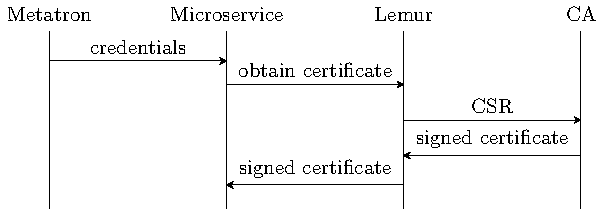
\includegraphics{images/related-work/netflix-provisioning.pdf}
%	\caption{Key provisioning of netflix using Lemur and Metatron~\cite{dias2020microservices}}
%	\label{fig:key_provisioning_netflix}
%\end{figure}

\section{Technologies}
\subsection{X509.Certificate}
X.509 certifcates bind the subject of a certificate to a public key.
They are used to assure the user of a certificate that the certificate's subject owns the corresponding private key.
The most significant advantage of certificates is that they can be exchanged using untrusted communication channels because the signature is not valid anymore when the content of a certificate is changed.
Therefore manipulations can be detected, and manipulated certificates can be declined~\cite{x509rfc}.

When a client wants to consume a service hosted on a server, it has to obtain the server's certificate.
If the client does not know the public key of the CA who signed the server's certificate, he has to obtain it.
Obtaining the public key often results in chains because the client may have to work his way up until he reaches a CA he trusts.
Such chains are also called certification paths~\cite{x509rfc}.

Depending on the version, a certificate can include more or less information.
The information is always stored inside the tbsCertificate, signatureAlgorithm, and signatureValue fields and can be expanded using extensions.
\begin{description}
	\item[TBSCertificate:] contains the data of the certificate, including the subject of the certificate, the issuer of the certificate, the public key of the subject, the validity period, and additional information~\cite{x509rfc}.
	\item[signatureAlogrithm:] stores the information, which cryptographic algorithm was used to sign the certificate.
		Algorithms are declared by their identifier, the "OBJECT IDENTIFIER".
		The most commonly used algorithms are the RSA algorithm and the Digital Signature Algorithm (DSA)~\cite{x509rfc}.
	\item[signatureValue:] contains the value of the digital signature.
		It is obtained by signing the content of the tbsCertificate, using the algorithm specified in the signatureAlgorithm field.
		The signature is used to verify the validity of the information embedded in the tbsCertificate field~\cite{x509rfc}.
\end{description}

\subsubsection{Certificate Revocation}
Certificate revocation is a considerable problem with certificates.
A certificate can be revocated for the following reasons: 
\begin{itemize}
    \item The Private key of the CA is compromised
    \item The Private key of the microservice is compromised
    \item The holder of the certificate is no longer the identity who requested the certificate 
    \item The CA finds out that the parameters provided in the CSR are invalid
\end{itemize}
The hardest part about the certificate revocation is informing all participants about the revocation of a certificate.
This is done using certificate revocation lists (CRL) or other revocation mechanisms.
The big downside of CRLS is that the CA has to store a list of certificates, which are revocated.
The clients have to retrieve this list whenever they establish a connection to a server, which causes high latencies.
The latencies can be reduced by caching.
Otherwise, caching also reduces the security because a certificate can be revocated during the lifetime of the cache.
Especially a case in which the CA does not respond to the CRL query is tough to handle.
Therefore certificate revocation is a significant downside of public-key-based authentication, even if the Online Certificate Status Protocol (OSCP) tries to remedy the situation\cite{dias2020microservices}.


\subsection{JSON Web Token}
A JSON Web Token (JWT) is a container that can carry authentication and authorization assertions and further information in a cryptographically safe manner.
An authentication assertion can be anything that authenticates the user.
Usually, usernames or e-mail addresses are used to identify a user uniquely.
An authorization assertion can be any information about the access permissions of a user.
For example, a JWT can include the information, whether the user is an admin or an unprivileged user~\cite{dias2020microservices}. 

\subsubsection{Structure}
A JWT is decomposed into the header, the payload, and the signature.
The three parts are concatenated and separated by a dot~\cite{jwtdocauth0}.
%A valid JWT could look like the JWT shown in figure~\ref{fig:myjwt}.
%\begin{figure}
%    \textcolor{red}{Header}.
%	\textcolor{blue}{Payload}.
%	\textcolor{darkgreen}{Signature} \\ \\
%    \textcolor{red}{eyJhbGciOiJIUzI1NiIsInR5cCI6IkpXVCJ9}.
%	\textcolor{blue}{eyJzdWIiOiIxMjM0NTY3ODkiLCJpYXQi\\OjE1MTYyMzkwMjIsInVzZXJuYW1lIjoiYmVuamFtaW4uZWxsbWVyIiwiZW1haWw\\iOiJiZW5qYW1pbi5lbGxtZXJAeWFob28uY29tIiwiYWRtaW4iOmZhbHNlfQ}.
%	\textcolor{darkgreen}{0ksqN7\\1oloNvq3IrY7w72uoTgPz9Gpn08p-KSbFulY0}
%    \caption{Sample JSON Web Token}
%    \label{fig:myjwt}
%\end{figure}

The \textbf{header} contains metadata related to the JWT, which is usually the type of the token and the signature algorithm.
The specification defines that only HS256\footnote{HMAC SHA-256} and none algorithm must be implemented by conforming JWT implementation.
It is recommended to additionally implement the algorithms RS256 and ES256\footnote{Elliptic Curve Digital Signature Algorithm (ECDSA) with 256-bit key}~\cite{jwtdocauth0, jwtrfc}.
The base64 encoded header is the first part of the JWT.

The \textbf{payload} is a set of registered and custom claims.
A claim is a piece of information about an entity.
The JWT specification defines registered claims, which are not mandatory for all cases but should provide a good starting point for a set of valuable claims to ensure interoperability.
The software architects can define custom claims on their own, depending on their needs.
The custom claims registered in the IANA registry are called public claims, and those not registered in the IANA registry are called private claims~\cite{jwtdocauth0, jwtrfc}.
The base64 encoded payload is the second part of the JWT.

The chosen signature algorithm signs the base64 encoded header, the base64 encoded payload, and a secret (only with symmetric encryption like HMAC).
The \textbf{signature} provides integrity for the message, and if it was signed with a private key, it additionally provides authentication~\cite{jwtdocauth0}.
The base64 encoded signature is the third part of the JWT.

\subsection{Transport Layer Security}
The Transport Layer Security (TLS) Protocol provides authentication, integrity, and confidentiality for the communication between two parties.
It consists of two layers, the handshake protocol and the record protocol~\cite{turnertls}.

\subsubsection{Handshake Protocol}
The handshake protocol is responsible for negotiating a cipher suite and for providing authentication using X.509 certificates.
The cipher suite declares the key exchange algorithm, the signature algorithm, the symmetric encryption algorithm, including the mode of the encryption algorithm and the hashing algorithm~\cite{turnertls, kurbatov2021design}.
The handshake varies on the key exchange method, but it can be separated into the following steps~\cite{krawczyk2013security}:
\begin{enumerate}
    \item The server and the client exchange Hello messages.
    \item The server sends its certificate to the client.
    \item The client sends a pre-master secret to the server.
    \item The client and the server finish the handshake, using the independently computed master secret.
\end{enumerate}

\subsubsection{Record Protocol}
The record protocol provides a secure channel for the secure communication of two parties.
This is done by using the algorithms declared in the cipher suite.
Confidentiality is assured, using symmetric encryption, and Message Authentication Codes (MAC) provide integrity~\cite{kurbatov2021design, krawczyk2013security}.

\subsubsection{mTLS} \label{sec:mtls}
TLS itself is also called one-way TLS because it helps the client to identify the server, but not the server to identify the client.
Therefore mTLS was introduced to provide authentication in both directions.
The client and the server must own a private/public key pair, so it is more suited for the communication between two systems and not between users and servers~\cite{dias2020microservices}. 
The authentication of the client is performed during the handshake.
When mTLS is used, the client has presents his certificate to the server, before transferring the pre-master secret.

\section{Conclusion}
This chapter described the fundamentals to understand the details and differences between the later described authentication mechanisms.
Furthermore, it was described why service-to-service authentication is needed and what additional mechanisms have to be implemented to secure a microservice deployment.

It is essential to understand that the whole system is compromised when one security mechanism does not work correctly.
For example, the authorization can be affected when the authentication is neglected.
Each service and each layer of the deployment has to be appropriately secured.
The problem with the microservice architecture is that one compromised service can be used to compromise other services.
Therefore, choosing the correct security mechanisms and understanding how they work is crucial. 

%Additionally, the possibility of outsourcing the authentication to a service mesh was discussed.
%The authentication mechanisms stay the same regardless of whether they are performed bythe services themselves or using the service mesh pattern.
%For the simplicity, it is assumed that the authentication mechanisms are performed by the services themselves in the following chapters.
